\documentclass[12pt]{article}
\usepackage{mathtext}
\usepackage{graphicx}
%\usepackage[cp1251]{inputenc}
\usepackage[russian]{babel}
\usepackage[T2A]{fontenc}
\usepackage[utf8]{inputenc}
%\linespread{2}
\usepackage{amsfonts}
\usepackage{amssymb}
\usepackage{amsmath}
\usepackage{pgfplots}
\usepackage{braket}
\usepackage{tikz}
\usepackage{float}
\headheight=0pt
\textwidth=15cm
%\oddsidemargin=2pt
%\topmargin=0pt
\textheight=22cm
%\topmargin=0pt
%\headsep=0pt
\newcommand{\nnn}{\bigskip}
\newcommand{\nn}{\medskip}
\newcommand{\n}{\smallskip}
\newcommand{\G}{\Gamma}
\renewcommand{\Im}{{\rm Im}}
\renewcommand{\d}{\delta}
\renewcommand{\b}{\beta}
\newcommand{\g}{\gamma}
%\newcommand{\mod}{{\rm mod}}
\newcommand{\sign}{{\rm sign}}
\newcommand{\Rev}{{\rm Rev}}
\newcommand{\grad}{{\rm grad }}
\newcommand{\card}{{\rm card}}
\newcommand{\ora}{{\rm or}}
\newcommand{\WH}{{\rm WH}}
\newcommand{\QFT}{{\rm QFT}}
\newcommand{\D}{\Delta}
\newcommand{\E}{{\rm E}}
\newcommand{\e}{\epsilon}
\newcommand{\FT}{{\rm FT}}
\newcommand{\ep}{\varepsilon}
\newcommand{\Qu}{{\rm Qu}}
\newcommand{\qu}{{\rm qu}}
\newcommand{\const}{{\rm const}}
\newcommand{\ar}{\longrightarrow}
\newcommand{\w}{\omega}
\newcommand{\s}{\sigma}
\newcommand{\la}{\lambda}
\renewcommand{\a}{\alpha}
\begin{document}
\title{Удалённое стимулирование сценариев  КЭД в модели Джейнса Каммингса Хаббарда на чистых состояниях }

\author{Андрей Кузьминский (1),\\  Юрий Ожигов (1,2)\\
{\it 
1. Московский Государственный Университет им. М.В.Ломоносова, 
} \\
{\it Факультет вычислительной математики и кибернетики,}
\\
{\it 2. Физико-технологический институт РАН им. К.А.Валиева}
\\ 
}
\maketitle

\begin{abstract}
Предложена модель удаленного стимулирования простых сценариев КЭД в системе оптических полостей, соединенных волноводами. Эта модель позволяет избежать избыточного описания состоянии в виде матрицы плотности и использовать только вектор чистого состояния, что дает возможность существенной экономии вычислительных ресурсов и позволяет моделировать на компьютере более сложные сценарии. 

\end{abstract}
\newpage

\section{Введение}
Дистантный перенос генетической информации является наиболее интригующим динамическим сценарием микромира . Эксперименты подобного рода проводились в нескольких лабораториях (см. в частности , работу \cite{mont} коллектива под руководством Люка Монтанье), что показало не только наличие эффекта но и нетривиальность тех условий которые требуются для его проявления . Последнее обстоятельство вызвало волну критики со стороны научной общественности (например работа  \cite{scept}); это говорит о важности как выяснения конкретных условий для дистантного переноса, так и самого механизма этого феномена. 

Вряд ли можно найти объяснение дистантного переноса, не привлекая квантовую механику, в частности, отдельных фотонов и их взаимодействие с атомами, что удобнее всего сделать в рамках модели Тависа-Каммингса-Хаббарда (TCH - \cite{TC}, \cite{T}), которая описывает взаимодействие многомодового поля с атомами, распределенными по оптическм полостям, соединенными волноводами.

Механизм, предлагаемый нами для объяснения дистантного переноса основан на существенном усилении энергии перехода между атомными состояниями при наличии большого числа фотонов данного перехода в окрестности атома; мы называем его индукцией перехода, а сам переход - индуцированным.

\section{Дистантный перенос состояний}

	Дистантный перенос квантовых состояний при перемещении только классической информации называется телепортацией. С пионерских работ \cite{Tel0},\cite{Tel} телепортация привлекает постоянный интерес как в связи с криптографией (см., например, \cite{Tel1}), так и сама по себе, как передача информации с помощью квантового канала связи. Это особенно актуально при организации квантовых сетей (\cite{netw}) и распределенных вычислений (\cite{gates}, \cite{transfer}). Есть также множество работ, посвященных конкретным физическим системам, в которых влияние дистантного переноса состояний важно: \cite{water},\cite{mont}, в частности, относящимся к биологической сфере - \cite{dna}, \cite{decoh},\cite{recogn}.

 Серьезной частью моделирования является описание декогерентности. Квантовый основное уравнение формально описывающее эволюцию квантовой системы с декогерентностью, не всегда подходит для практического моделирования в связи с проблемой сложности. Использование для такого моделирования матрицы плотности не является оптимальным шагом из за избыточности такого описания. Случайность в матрице плотности подразделяется на классическую в виде весов квантовых состояний, и квантовую, заключенную в самих этих состояниях, что и создает избыточность, ведущую к перерасходу компьютерной памяти из за необходимости хранить матрицу вместо вектора. 

Имеется цикл работ посвященных модификация квантового основного уравнения для с учетом данной трудности- \cite{qcl},\cite{lindbl}. Мы будем использовать модификацию модели TCH с использованием только вектора состояния в метро вместо матрицы плотности.
 Идея такого подхода восходит к работам по квантовому отжигу (\cite{1}, а также более ранняя \cite{2}), в которых разыскивался глобальный минимум некоторой функции. В нашем случае виртуальный вектор состояния предназначен не для математической задачи поиска экстремума, а для моделирования естественного процесса.

Однако при постоянном гамильтониане такое описание приведет к хаосу из за отсутствия однонаправленного характера динамики. Именно введение операторов декогерентности в квантовом основном уравнении создает такую однонаправленность, платой за что и является избыточность описания. 

Мы рассмотрим более простой способ создания однонаправленного характера основанный на  гамильтониане Джейнса Каммингса Хаббарда. Этот гамильтониан описывает динамику квантовых состояний ансамблей двухуровневых атомов распределенных по оптическим полостям соединенным волноводами. Наша модель позволяет представлять динамику ансамблей без оптических полостей, когда фотоны удаляются из одной локации и могут попасть в другую. Это перемещение фотонов при определенных условиях может создать интересный эффект удаленного стимулирования сценариев квантовой электродинамики на примере которых мы продемонстрируем возможности нашей модели. 



 


\section{Простейший пример фотонного трансфера динамики }

Дистанционный трансфер квантовых состояний (см., например, \cite{transfer}) является важнейшим эффектом, роль которого пока еще не полностью ясна. Мы рассмотрим родственный эффект удаленного стимулирования сценариев КЭД, и проиллюстрируем на его примере эффективность чисто унитарной модели.

%Для исключения матрицы плотности мы должны представлять эволюцию только в виде унитарной динамики . Однако такая динамика с постоянным гамильтонианом всегда приводит к хаосу из-за обратимости процесса что не дает возможность исследовать распределение вероятностей. Выходом является изменения параметров гамильтониана со временем. В нашем случае это будет вариация проводимости волноводов которые соединяют оптические полости в модели Джеймса Каммингса Хаббарда. Такая вариация дает эффект измерения в виде улета фотонов, однако не требует введение матрицы плотности или ее аналогов. 

Рассмотрим простейший пример перехода между уровнями в одной полости, индуцированного фотонами, приходящими из аналогичных систем в окружении. Основой будет конфигурация, изображенная на рисунке \ref{fig:f1a}, где мы рассматриваем трансфер фотонов из полостей $1, 2, … , n$ в полость $0$. Начальное состояние выберем вида $|0,1,1,...,1\rangle$, где нумерация полостей начинается с нуля. Унитарная осцилляция при постоянном гамильтониане Джеймса Каммингса Хаббарда для системы полостей в левой части рисунка \ref{fig:f1a} ведет к чередованию состояний $|0,1,1,...,1\rangle\leftrightarrow |n,0,0,...,0\rangle$. Таким образом, фотоны, покидающие полости $1,2,...,n$ все оказываются в полости $0$. Если разместить в полостях по одному атому так что переход, индуцированный фотоном данной моды происходит в полости $0$ гораздо медленнее чем в остальных полостях, то этот переход может существенно ускориться из за наличия многих фотонов в полости $0$. 

Разобьем переход $|0,1,1,...,1\rangle\leftrightarrow |n,0,0,...,0\rangle$ на 2 участка с одинаковой продолжительностью. 1 переход $|0,1,1,...,1\rangle\rightarrow |n,0,0,...,0\rangle$ будет соответствовать наполнению полости ноль, а 2 переход $|0,1,1,...,1\rangle\leftarrow |n,0,0,...,0\rangle$ будет соответствовать стоку фотонов в полость sink. Последний процесс можно отождествить с вылетом фотонов из полости 0 в окружающее пространство. На этом сценарии завершается . Наличие фотонов моды резонаторов начиная с 1 усиливает соответствующий переход так что он начинает превалировать перед собственным переходом в полости ноль - \ref{fig:f2a} внизу. Это и есть удаленный трансфер динамики . 

Возможно также присутствие в целевой локации нескольких 3 уровневых систем как показано внизу рисунка \ref{fig:f2a}. В этом случае при симметричных характеристиках однотипных систем целесообразно использовать новый базис, состоящие из взвешенных состояний однотипных систем, как показано в книге Ожигова. Наконец, можно рассмотреть удаленную индукцию динамических сценариев на много уровневых системах. Такой эффект применим, например, в описании процесса образование кристаллов льда. Здесь каждый уровень соответствует определенному частичному кристаллу, так что в большой массе молекул воды будет происходить удаленная индукция динамических сценариев совершенно определенного вида приводящая к однотипным кристаллам льда. 

Вот какие вычислительные задачи в связи с этим возникают . 

1 . Что будет если начинать не с состояния $|0,1,1,...,1\rangle$ а с состояния $|1,1,1,...,1\rangle$ . 

2. что будет если полости 1,2 и так далее также связано волноводами . 

3 . Произвести полный расчет трансфера динамики с учетом подавления основного перехода в нулевой полости индуцированном переходом из полостей 1,2,...

4. Распространить схему трансфера динамики на многоуровневые системы . В частности , произвести расчеты для образование нано снежинок в воде и синтеза днк .




\begin{figure}[H]
\centering
\includegraphics[scale=1.3]{f1a.jpg} 
\caption{ Общая схема удаленного индуцирования динамического сценария }
\label{fig:f1a}
\end{figure}

\begin{figure}[H]
\centering
\includegraphics[scale=1.3]{f2a.jpg} 
\caption{ Трансфер динамического сценария с подавлением базисного перехода на уровень В}
\label{fig:f2a}
\end{figure}



Численные характеристикой удаленной стимулирования является вероятность попадание фотонов в sink A по сравнению c sink B . При отсутствии полостей справа (их можно назвать стимулирующими полостями) наполнение sink B преобладает. Присутствие стимулирующих полостей создает преимущество наполнение sing A . Этот эффект мы назовем удаленным стимулированием . 

{\bf Что нужно вычислить с помощью моделирования на компьютере }. 

1. Установить эффект удаленного стимулирования. 

2. Выявить зависимость эффекта удаленного стимулирования от числа стимулирующих полостей. 

3. Выяснить зависимость эффекта удаленного стимулирования от структуры связей полостей волноводами.  

4. Установить эффект удаленного стимулирования для многоуровневых систем , в частности , для систем из 6 уровней , которые имитируют нано снежинку . 

\section{Удалённое стимулирование коллективных сценариев }

Рассмотрим сетку из волноводов соединяющих полости находящиеся вершина целочисленной сетки . Рассмотрим систему полостей близких состоящих из 7 полостей - одна в центре и 6 по бокам; пусть также аналогичная система имеется на некотором расстоянии . Наша цель состоит в том , чтобы перенести коллективная сценарий из 1 системы во 2 систему. 

В полостях из 1 системы мы разместим по одному фотону которые будут стимулировать наименее вероятный переход в лямбда системе атома. В полостях из 2 системы мы разместим по одному атому данного типа. Подобно тому что было в предыдущем параграфе . Задача состоит в том , чтобы найти насколько повышается вероятность априори слабого перехода в результате прилета фотонов из 1 системы (см. рисуное \ref{fig:fa3}). Здесь можно использовать базисное состояние из системы коллективных осцилляций (смотри книгу ). Специфика задачи состоит в огромном числе базисных состоянии возникающим из-за пространственного удаления 1 и 2 системы . При моделировании надо будет использовать метод отбора рабочей области . Это очень хорошая модельная задачи на метод отбора . 

\begin{figure}[H]
\centering
\includegraphics[scale=1.7]{fa3.jpg} 
\caption{ Индукция коллективного сценария}
\label{fig:fa3}
\end{figure}

\section{Результаты моделирования}

Было промоделировано несколько конфигураций систем с трёхуровневыми атомами.

Первая конфигурация состояла из 0 полости с n атомами в состояниях с наивысшей энергией и 1 полости с m фотонами с переходом А из  рисунка \ref{fig:f2a}. Результаты показали лишь незначительное отклонение оригинального сценария без 1 полости с фотонами. С улётом же фотонов итогового изменения нет. Причина данного результата в том, что фотоны с модой перехода А усиливают обратный переход в состояние с наивысшей энергией, у которой наиболее вероятен переход B.
Вторая конфигурация оказалась успешной - 0 полость с n атомами в состояниях с наивысшей энергией у которых возможны все переходы и 1 полость с m атомами в состояниях с наивысшей энергией, у которых возможен только переход А. В данной конфигурации отчётливо проявляется эффект удалённого стимулирования. Ниже приведены результаты с единичным количеством атомов на полость (увеличение их количества не влияет на итоговый результат, за исключением замедления роста вероятности желаемого состояния $|A\rangle$. Сами же пределы не меняются) - только 0 полость на рисунке \ref{fig:orig} и результат с эффектом удалённого стимулирования на рисунке \ref{fig:distant}. 

\begin{figure}[H]
\centering
\includegraphics[scale=1.7]{orig.png} 
\caption{ Индукция коллективного сценария}
\label{fig:orig}
\end{figure}

\begin{figure}[H]
\centering
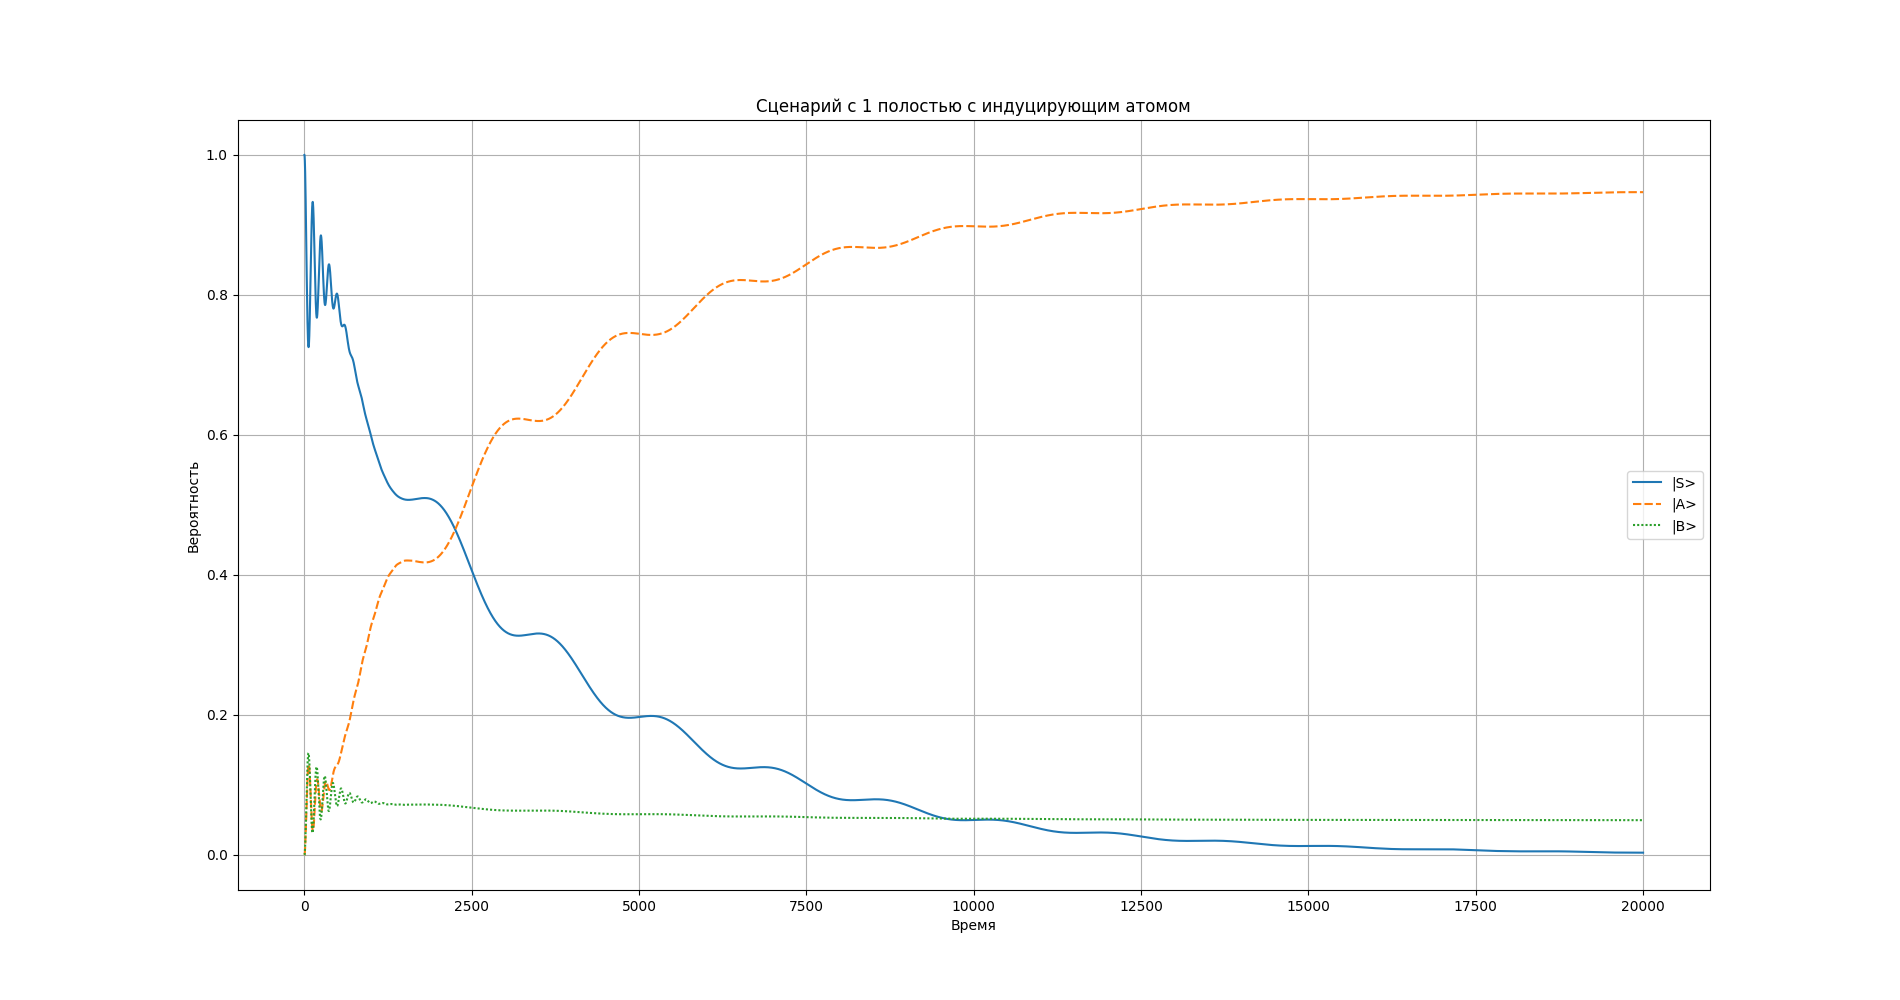
\includegraphics[scale=1.7]{distant.png} 
\caption{ Индукция коллективного сценария}
\label{fig:distant}
\end{figure}

Далее будут продемонстрированы зависимости данного эффекта от различных параметров. Сначала в зависимости от разницы энергий между энергиями перехода А и B на Рис. \ref{fig:en_time} и Рис. \ref{fig:en_prob_diff}. На Рис. \ref{fig:en_time} продемонстрирован момент времени, когда вероятность перехода А становится больше всех остальных исходов. На Рис. \ref{fig:en_time} выведена разница вероятностей при устремлении в бесконечность (то есть ассимптоты) перехода А и перехода B. На них виден характер данного эффекта в зависимости от разницы частот уровней А и В. Видно, что данный эффект оказывается довольно стабильным при большом диапозоне разниц энергий и перестаёт действовать в данной ситуации, когда энергия перехода на уровень В превышает перехода на уровень А в ?? раз.

\begin{figure}[H]
\centering
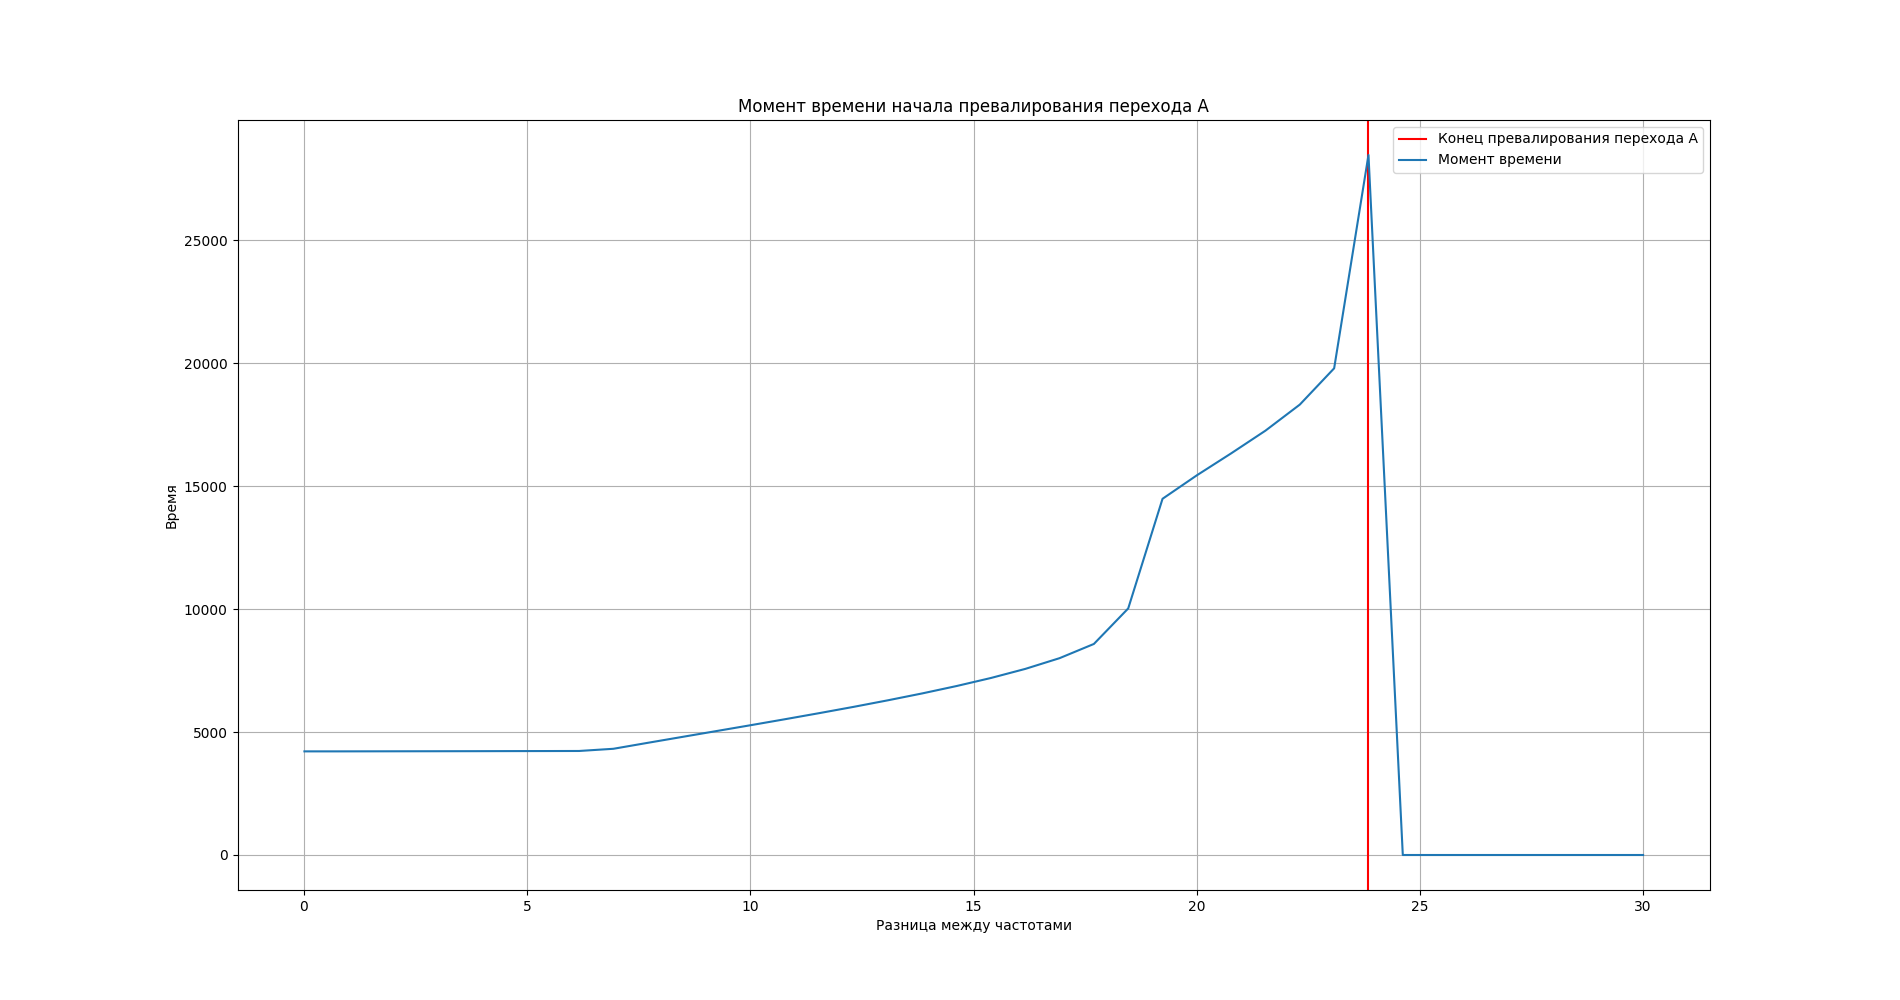
\includegraphics[scale=1.7]{w_time.png} 
\caption{ Индукция коллективного сценария}
\label{fig:en_time}
\end{figure}

\begin{figure}[H]
\centering
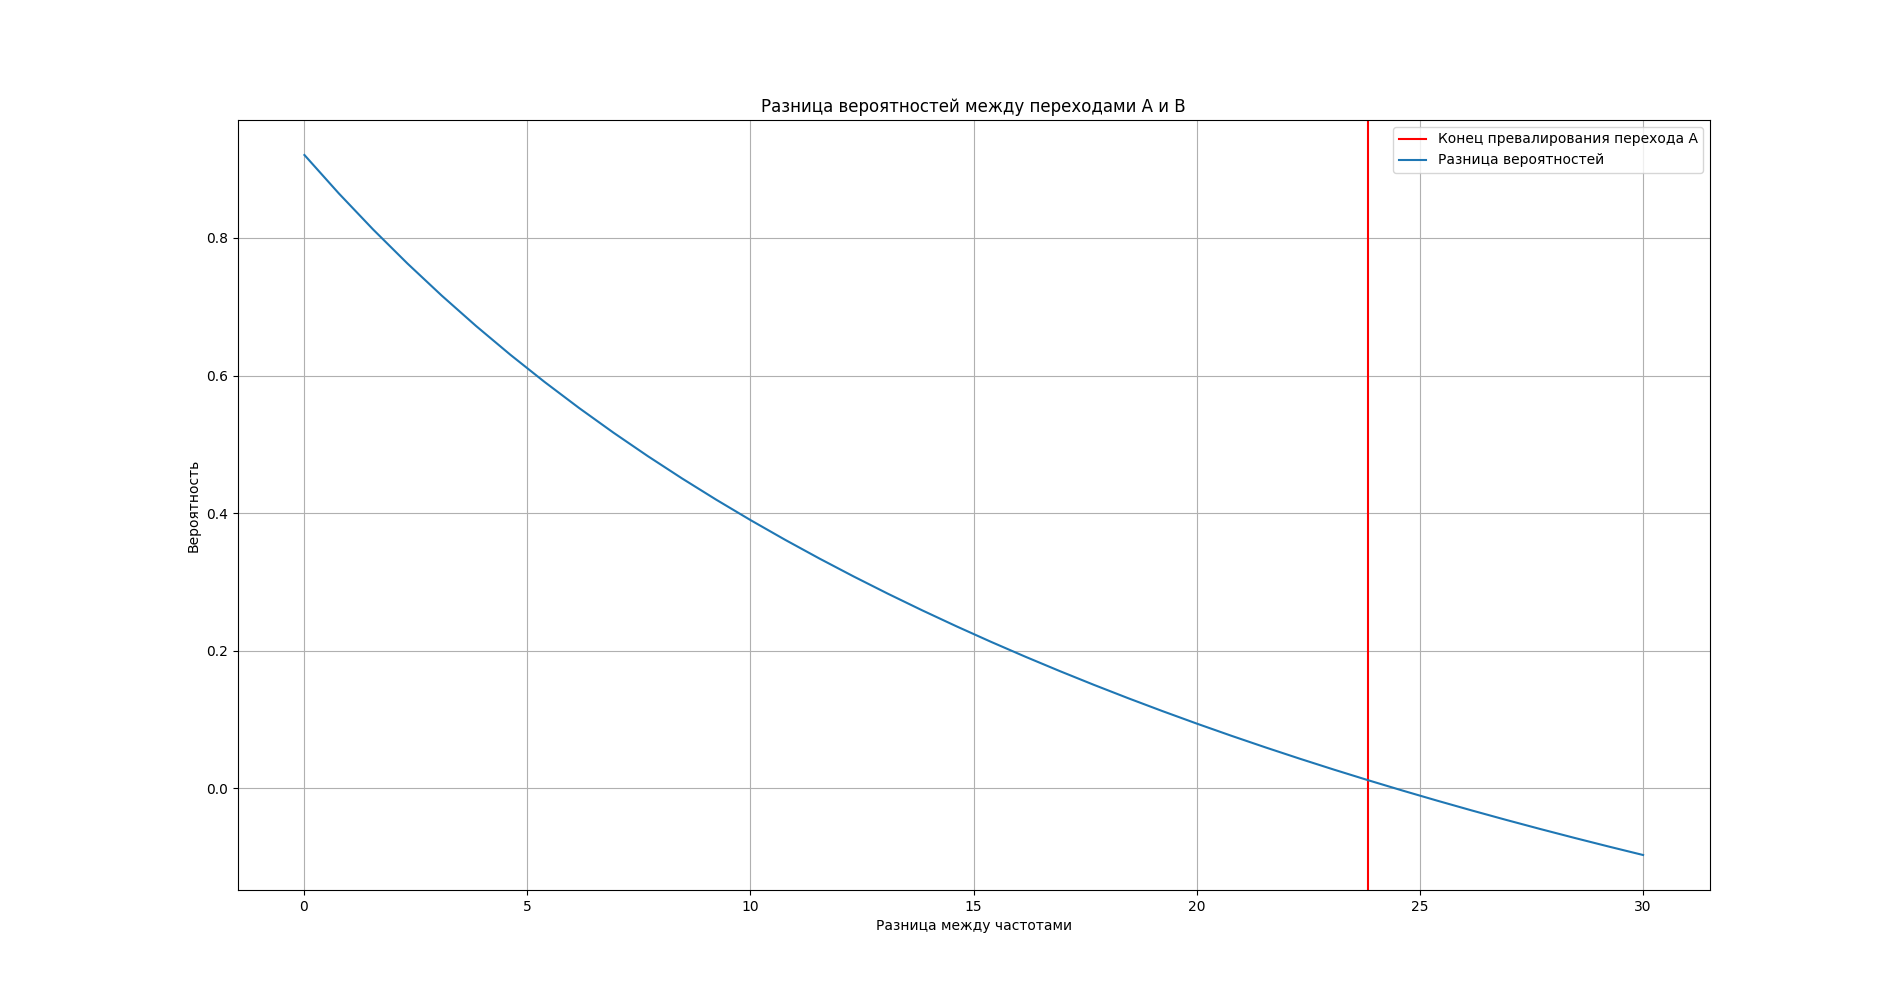
\includegraphics[scale=1.7]{w_prob_diff.png} 
\caption{ Индукция коллективного сценария}
\label{fig:en_prob_diff}
\end{figure}

Теперь рассмотрим зависимость от интенсивностей волновода между 0 и 1 полостью, а также от интенсивности утечки фотонов из 0 полости. На Рис. \ref{

\begin{figure}[H]
\centering
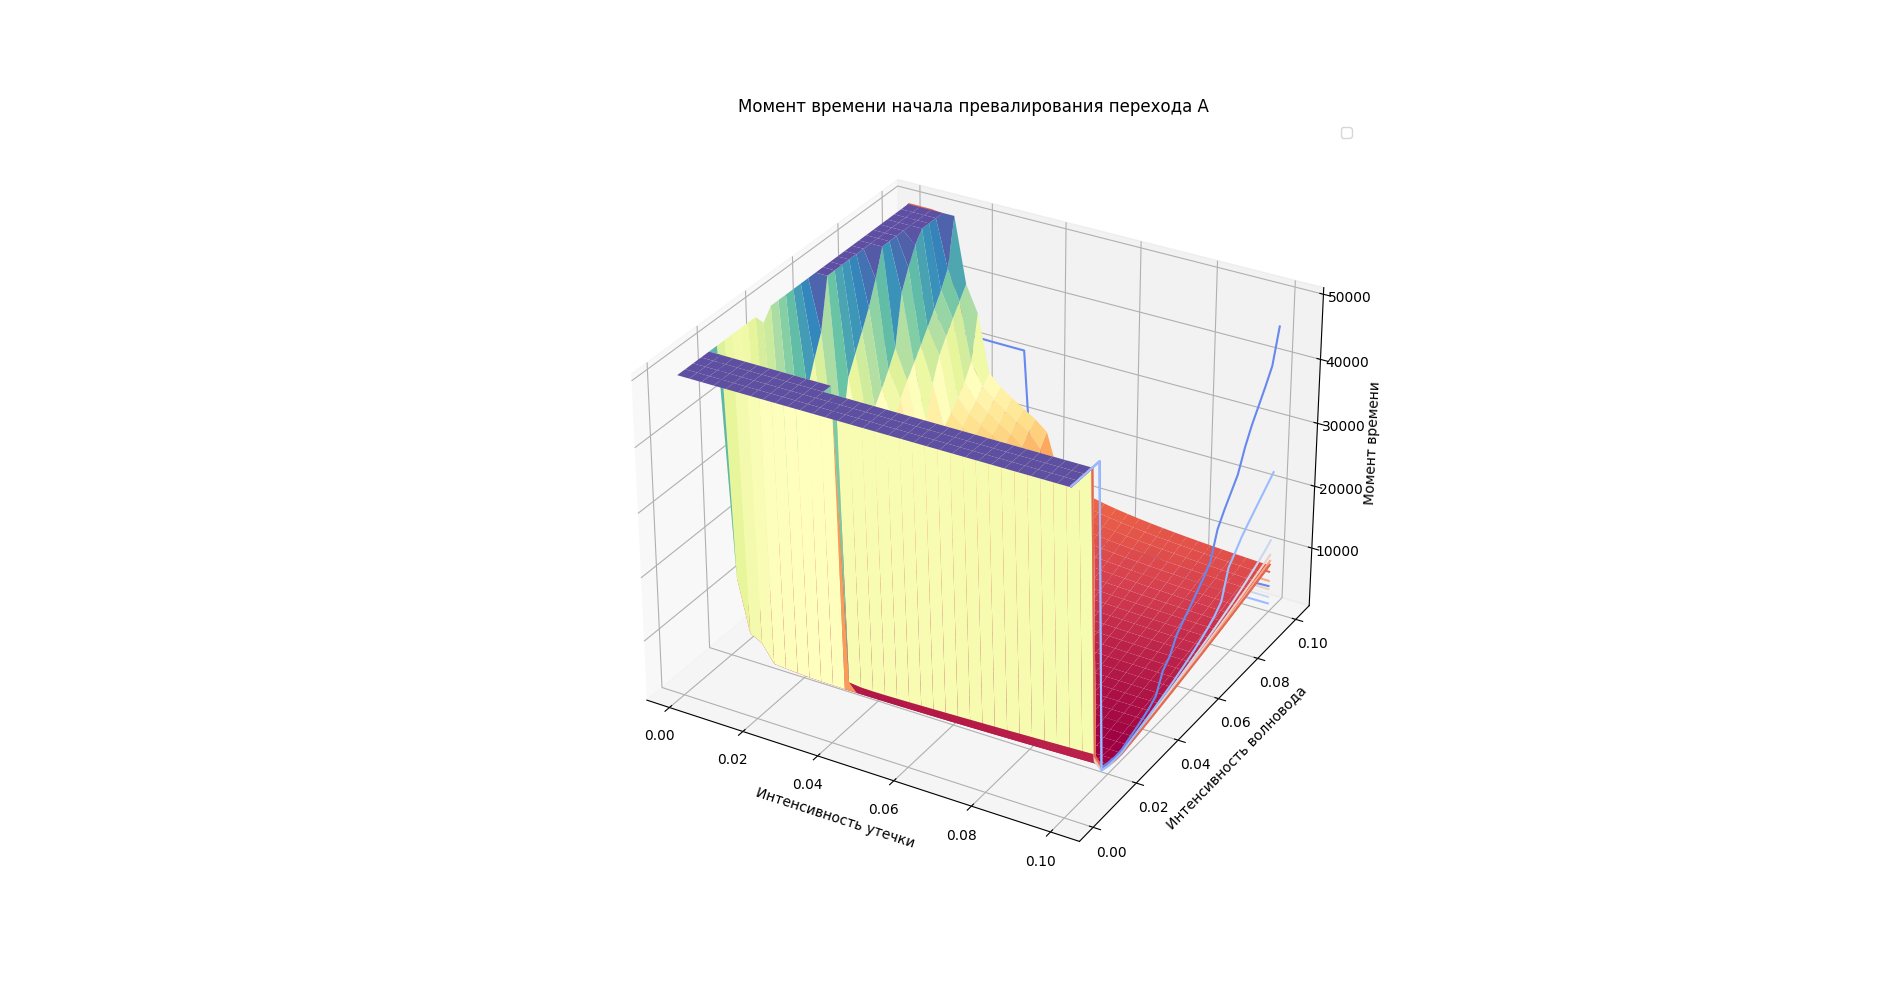
\includegraphics[scale=1.7]{wave_time.png} 
\caption{ Индукция коллективного сценария}
\label{fig:en_time}
\end{figure}

\begin{figure}[H]
\centering
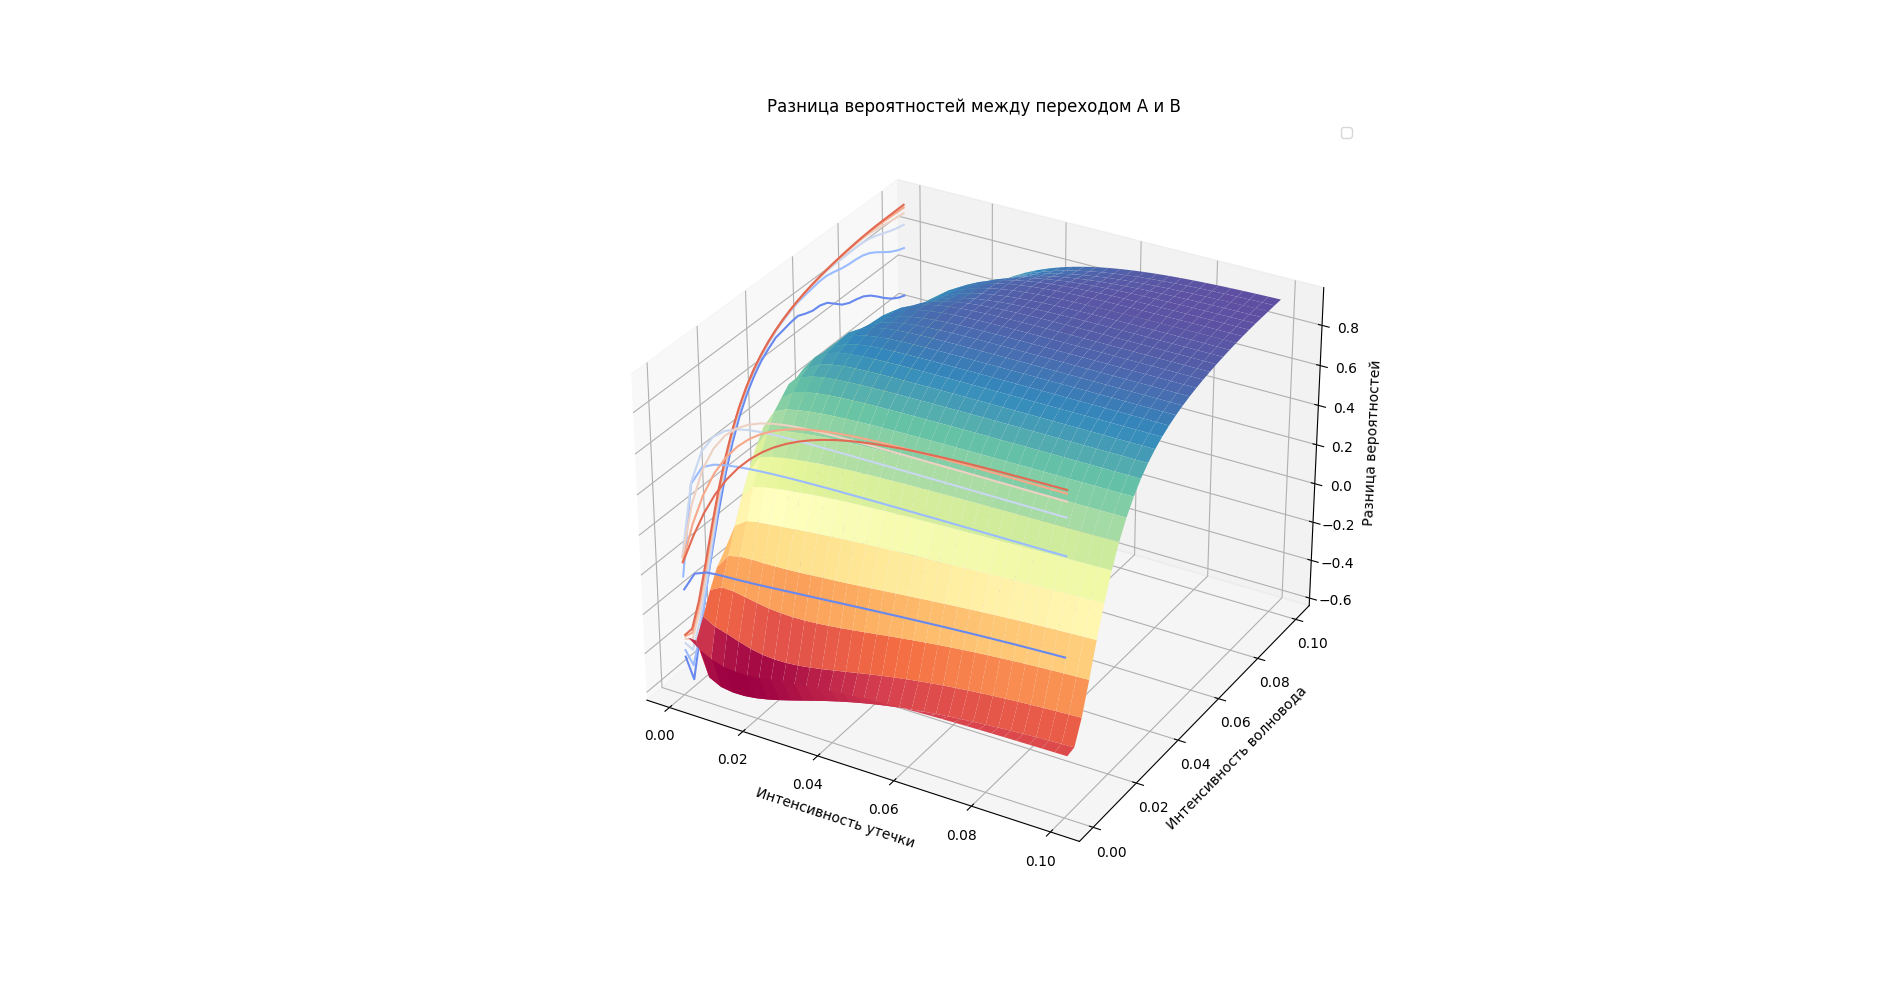
\includegraphics[scale=1.7]{wave_prob_diff.png} 
\caption{ Индукция коллективного сценария}
\label{fig:en_prob_diff}
\end{figure}

\begin{thebibliography}{99}
\bibitem{netw} Alexander Kolar, Allen Zang, Joaquin Chung, Martin Suchara, Rajkumar Kettimuthu, Adaptive, Continuous Entanglement Generation for Quantum Networks, IEEE INFOCOM 2022-IEEE Conference on Computer Communications Workshops (INFOCOM WKSHPS), pp. 1-6. IEEE, 2022.
\bibitem{gates}Guillermo F. Peñas, Ricardo Puebla, Tomás Ramos, Peter Rabl, Juan José García-Ripoll, Universal deterministic quantum operations in microwave quantum links, PhysRevApplied.17.054038 (2022).
\bibitem{transfer} G. D. de Moraes Neto, F. M. Andrade, V. Montenegro, S. Bose, Quantum state transfer in optomechanical arrays, Phys. Rev. A 93, 062339 (2016).
%\bibitem{transfer}G. D. de Moraes Neto, F. M. Andrade, V. Montenegro, S. Bose, Quantum state transfer in optomechanical arrays,  Phys. Rev. A 93, 062339 (2016).
\bibitem{TC}E. T. Jaynes, F. W. Cummings, “Comparison of quantum and semiclassical radiation theories
with application to the beam maser”, Proc. IEEE, 51:1 (1963), 89–109.
\bibitem{T} M. Th. Tavis, A Study of an N Molecule Quantized-Radiation-Field Hamiltonian, Dissertation,
arXiv: 1206.0078.
\bibitem{Tel1}Hannah McAleese, Mauro Paternostro, Critical assessment of information back-flow in measurement-free teleportation, Entropy 26, 780 (2024).
\bibitem{Tel}Charles H. Bennett, Gilles Brassard, Sandu Popescu, Benjamin Schumacher, John A. Smolin, William K. Wootters, Purification of Noisy Entanglement and Faithful Teleportation via Noisy Channels, hys.Rev.Lett.76:722-725,1996.
\bibitem{Tel0}Gilles Brassard, Teleportation as a quantum computation, Physica D120 (1998) 43-47.
\bibitem{scenario} Alexander Streltsov, Swapan Rana, Manabendra Nath Bera, Maciej Lewenstein, Towards resource theory of coherence in distributed scenarios, Phys. Rev. X 7, 011024 (2017).
\bibitem{water}Cowan, M.L., Bruner, B.D., Huse, N., Dwyer, J.R., Chugh, B., Nibbering, E.T., Elsaesser, T., Miller, R.J. 2005. Ultrafast memory loss and energy redistribution in the hydrogen bond network of liquid H2O. Nature 434, 199–202.
\bibitem{mont}Montagnier, L., Aïssa, J., Ferris, S. et al. Electromagnetic signals are produced by aqueous nanostructures derived from bacterial DNA sequences. Interdiscip Sci Comput Life Sci 1, 81–90 (2009). https://doi.org/10.1007/s12539-009-0036-7
\bibitem{scept} Andy Coghlan, Scorn over claim of teleported DNA, Newscientist, Phys \&Math, 12 January 2011, 2795
\bibitem{dna} Zhen Feng, Zhen-Wei Gao, Lian-Ao Wu, Hao Tang, Ke Sun, Cheng-Qiu Hu, Yao Wang, Zhan-Ming Li, Xiao-Wei Wang, Yuan Chen, En-Ze Zhang, Zhi-Qiang Jiao, Xiao-Yun Xu, Jun Gao, Ai-Lin Yang, Xian-Min Jin, Photonic Newton's Cradle for Remote Energy Transport, Phys. Rev. Applied 11, 044009 (2019).
\bibitem{decoh} Ignacio Gustin, Chang Woo Kim, David W. McCamant, Ignacio Franco, Mapping Electronic Decoherence Pathways in Molecules, PNAS. 120, e2309987120 (2023).
\bibitem{recogn}Onur Pusuluk, Gokhan Torun, Cemsinan Deliduman, Quantum entanglement shared in hydrogen bonds and its usage as a resource in molecular recognition,  Modern Physics Letters B 32, 1850308 (2018).
\bibitem{qcl}Cesare Tronci, David Martínez-Crespo, François Gay-Balmaz, Entropy functionals and equilibrium states in mixed quantum-classical dynamics, arXiv:2501.18587
\bibitem{lindbl}Dhrumil Patel, Mark M. Wilde, Wave Matrix Lindbladization I: Quantum Programs for Simulating Markovian Dynamics, Open Systems \& Information Dynamics, Vol. 30, No. 02, page 2350010 (June 2023)
Related DOI: https://doi.org/10.1142/S1230161223500105
\bibitem{1} Кадоваки, Т.; Нисимори, Х. (1998). "Квантовый отжиг в поперечной модели Изинга". Phys. Rev. E. 58 (5): 5355. arXiv:конд-мат /9804280. Bibcode:1998PhRvE..58.5355К. doi:10.1103/PhysRevE.58.5355. S2CID 36114913
\bibitem{2}Аполлони, Бруно; Карвалью, Мария К.; Де Фалько, Диего (1989). "Квантовая стохастическая оптимизация". Stoc. Проц. Приложение. 33 (2): 233–244. doi:10.1016/0304-4149(89)90040-9

\end{thebibliography}
\end{document}



%\bibitem{0}Квантовые аспекты жизни, https://doi.org/10.1142/p581 | Сентябрь 2008
Страницы: 468, Под редакцией: Дерек Эбботт (Университет Аделаиды, Австралия), Пол К. В. Дэвис (Университет штата Аризона, США) и Арун К. Пати (Институт физики, Орисса, Индия)
\bibitem{1} Кадоваки, Т.; Нисимори, Х. (1998). "Квантовый отжиг в поперечной модели Изинга". Phys. Rev. E. 58 (5): 5355. arXiv:конд-мат /9804280. Bibcode:1998PhRvE..58.5355К. doi:10.1103/PhysRevE.58.5355. S2CID 36114913
\bibitem{2}Аполлони, Бруно; Карвалью, Мария К.; Де Фалько, Диего (1989). "Квантовая стохастическая оптимизация". Stoc. Проц. Приложение. 33 (2): 233–244. doi:10.1016/0304-4149(89)90040-9
\bibitem{3}М.А.Зенкова, Г.Г.Карпова, Несовершенные комплексы нуклеиновых кислот и их биохимическое проявление, Успехи Химии, 62 (4),  стр. 414-435, 1993
\bibitem{4}Стилвелл В. Мембранный транспорт. Введение в биологические мембраны. 2016:423-51. doi: 10.1016/B978-0-444-63772-7.00019-1. Epub 2016, 15 июля. PMCID: PMC7182109.
\bibitem{QComputations} https://github.com/KuzmaLine/QComputations
\bibitem{Realization} https://github.com/KuzmaLine/emulation
\bibitem{B}R. Boyd, Nonlinear optics, 
Нелинейно-оптические процессы третьего порядка. 2020, Elsevier Science \& Technology; pp. 636
ISBN 10: 0128110031 ISBN 13: 9780128110034
\bibitem{K}Ханин Я.И.  Лекции по квантовой радиофизике, 
Tags: электротехника   квантовая радиотехника   лекции   радиофизика   квантовая физика  
ISBN: 5-8048-0057-4 Year: 2005
\bibitem{S}А.В.Линев, А.М.Сатанин
ТЕХНИКА РЕШЕНИЯ НЕСТАЦИОНАРНОГО УРАВНЕНИЯ
ШРЕДИНГЕРА С ИСПОЛЬЗОВАНИЕМ ПАРАЛЛЕЛЬНОЙ ВЕРСИИ
МЕТОДА РУНГЕ-КУТТА, Нижегородский государственный университет им. Н.И. Лобачевского
Национальный исследовательский университет, Учебно-методическая разработка по дисциплине
"Квантовая механика" 2014.
\bibitem{11}    Булавин,  H.B.  Выгорницкий,  Н.И.  Лебовка
 Компьютерное  моделирование  физических  систем:  Учебное
пособие  /  JI.A.  Булавин,  Н.В.  Выгорницкий,  Н.И.  Лебовка  -
Долгопрудный:  Издательский  Дом  «Интеллект»,  2011.  —  352  с.
 ISBN  978-5-91559-101-0


\end{thebibliography}
\end{document}



